\chapter{Diplexer}
\label[appendix]{sec:annex_a}


\begin{figure}[b]
    \centering
    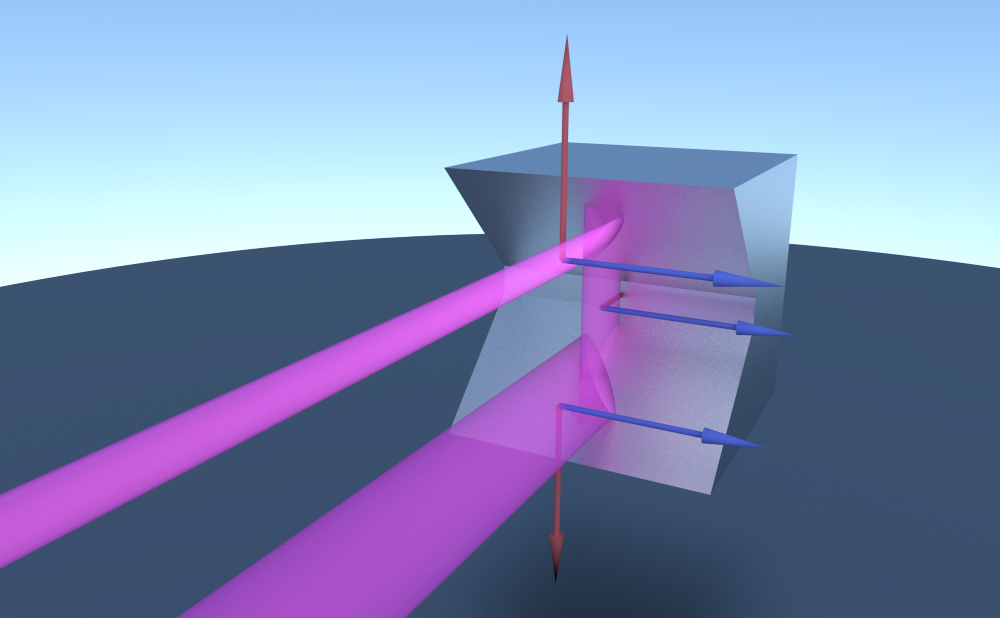
\includegraphics[width=\textwidth]{rooftop_polar_lowres}
    \caption{Rooftop mirrors flip the direction of one polarization and keep the other constant.}
    \label{fig:rooftop_polar}
\end{figure}

\begin{figure}[b]
    \centering
    \input{diplexer.pdf_tex}
    \caption{Principle of the Martin--Puplett interferometers used in HIFI Bands~3, 4, 6 and 7.}
    \label{fig:diplexer}
\end{figure}

The diplexer units of HIFI contain a Martin--Puplett interferometer~\parencite{martin1982polarizing} composed of one wire-grid polarizer and two rooftop mirrors.
\Cref{fig:diplexer} illustrates its principle.
The input wave (sky or LO, purple on the figure) is split in two by the wire grid polarizer.
Each half (blue and red) carries one half of the power and travels down one arm of the interferometer where it eventually meets a rooftop mirror.
The rooftop mirrors are oriented so that the input waves are reflected back toward the grid with their polarization rotated by~\SI{90}{\degree}: if the first encounter with the grid is reflective then the second is transmissive and vice versa.
The two waves propagating toward the mixer can be seen as a single output wave (principle of superposition).
The phase difference between the two waves determines the polarization of that output wave.
On the figure, the dots on the paths of the wave represent the crests of that wave;
we can see that the blue and red dots are not in phase when they reach the mixer.
The phase difference depends on the the length of the mobile arm (red) and the frequency of the wave.

An ideal diplexer is modeled by
\begin{align}
    G_\text{sky}(f)
    &=
    \cos
    \left(
        2 \pi
        \frac{df}{c}
    \right)^2
    \\
    G_\text{LO}(f)
    &=
    1 - G_\text{sky}(f)
    \label{eq:diplexer_coupling_model}
\end{align}
with $G_\text{sky}$ and $G_\text{LO}$ the coupling of the mixer to the sky and the LO,
$f$ the wave frequency,
$d$ the length difference between the two arms of the interferometer,
and $c$ the speed of light in the propagation medium (vacuum in our case).

This frequency-dependence implies that the coupling of the mixer to the LO and the sky cannot be optimal over a wide range of frequencies.
In HIFI, the nominal pathlength difference is chosen so that the mixer is maximally coupled to the LO at the LO frequency~$f_\text{LO}$,
and to the sky at $f_\text{LO} \pm \SI{6}{\giga\hertz}$.
This value of~\SI{6}{\giga\hertz} corresponds to the center of the bandwidth of the mixer, which ranges from \num{4} to \SI{8}{\giga\hertz}.
As a result, the coupling of the mixer to the sky is optimal at the center of the spectrum.
This is illustrated by the diplexer coupling model on the top plot of~\cref{fig:diplexer_ideal}.
In that ideal case, the sideband ratio SBR defined as
\begin{equation}
    \text{SBR} =
    \frac{
        G_\text{USB}
    }{
        G_\text{LSB} + G_\text{USB}
    }
\end{equation}
is constant over the whole bandwidth and equals \num{0.5}, which means that the mixer couples to both sidebands equally, as shown on the bottom plot of~\cref{fig:diplexer_ideal}.

At the edges of the sidebands, the coupling to the sky is lower and the coupling to the LO is higher.
Since the LO is a source of thermal noise, the signal-to-noise ratio decreases toward the edges of the spectrum.
This can be seen on the baseline of~\cref{fig:co98_full_bandwidth}.

\begin{figure}
    \centering
    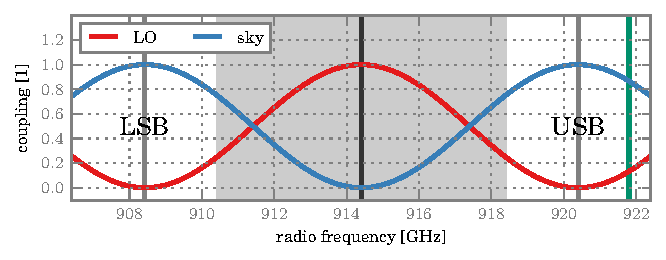
\includegraphics{diplexer_coupling_ideal}
    \caption*{
        Coupling of the mixer to the LO and the sky for an optimally-tuned diplexer.
        The mixer--LO coupling is maximal at the LO frequency
        (black vertical line at~\SI{914.4045}{\giga\hertz}).
        The mixer--sky coupling is maximal at the center of the lower and upper sidebands (gray vertical lines LSB and USB).
    }
    \bigskip
    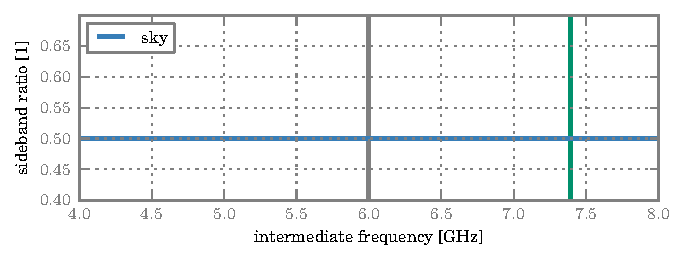
\includegraphics{diplexer_sbr_ideal}
    \caption*{
        Sideband ratio of the mixer--sky coupling for an optimally-tuned diplexer.
        The constant sideband ratio of \num{0.5} indicates that the LSB and the USB contribute in equal measure to each channel of the spectrum.
    }
    \caption{
        Model of the coupling and the sideband ratio for an optimally-tuned diplexer.
        The green vertical lines show the rest frequency of the \transition{CO}{8}{7} transition.
        The LO frequency is~\SI{914.4045}{\giga\hertz}.
        The difference in length of the two arms of the diplexer is~\SI{12.5405}{\milli\meter}.
    }
    \label{fig:diplexer_ideal}
\end{figure}

Because each LO frequency requires its own optical pathlength difference, 
one of the rooftop mirrors can be translated.
This translation is commanded by an electric current applied to an actuator.
The equation relating~$I$, diplexer actuator current in milliampere, to~$d$, interferometer arm length difference in millimeter, is
\begin{equation}
    d = d_0 + 27.5 \frac{2\pi}{360}(a I^2 + b I)\text{.}
\end{equation}
The currents $I$ are given in~\cref{tab:los_and_dacs}.
The remaining parameters $d_0$, $a$ and $b$ are given in~\cref{tab:diplexer_params}.
These parameters are very well known and have remained constant (sub-micrometer precision) during the entire mission \parencite{mueller2014flight}.

\begin{table}
    \centering
    \begin{tabular}{cccc}
        \toprule
        mixer &
        $a$ [\si{\degree\per\milli\ampere\squared}]
        &
        $b$ [\si{\degree\per\milli\ampere}]
        &
        $d_0$ [\si{\milli\meter}]
        \\
        \midrule
        3h    &  \num{-0.003991} & 0.1976 & 12.3354\\
        3v    &  \num{-0.004821} & 0.2155 & 12.1231\\
        4h    &  \num{-0.004348} & 0.1722 & 12.3490\\
        4v    &  \num{-0.003553} & 0.1791 & 12.5395\\
        6h    &  \num{-0.002401} & 0.1735 & 21.0532\\
        6v    &  \num{-0.005408} & 0.2100 & 20.8718\\
        7h    &  \num{-0.002272} & 0.1661 & 20.7954\\
        7v    &  \num{-0.002757} & 0.1586 & 20.7666\\
        \bottomrule
    \end{tabular}
    \caption{Parameters used to convert diplexer actuator currents to interferometer arm length difference.
    We use the mixers 3h and 4h in our study.}
    \label{tab:diplexer_params}
\end{table}
